\documentclass[conference]{IEEEtran}

\usepackage{cite}
\usepackage{graphicx}
\usepackage{amsmath}
\usepackage{booktabs}
\usepackage{multirow}
\usepackage{array}
\usepackage{url}
\usepackage{float}
\usepackage{balance}
\usepackage{xcolor}
\usepackage{hyperref}
\hypersetup{colorlinks=true,linkcolor=blue,citecolor=blue,urlcolor=blue}
\graphicspath{{figures/}}

\title{Data-Driven AI-Based Scholarship Recommendation and Eligibility Analysis System Using Natural Language Processing and Machine Learning}

\author{\IEEEauthorblockN{Author Name}
\IEEEauthorblockA{Department of Data Science and Machine Learning\\
Institution Name\\
Tamil Nadu, India\\
Email: author@email.com}}

\begin{document}
\maketitle

\begin{abstract}
Scholarships can help students continue their education, but finding relevant opportunities can be difficult because schemes are described across different departments, institutions, welfare boards, and portals. Their requirements may depend on education level, course, academic performance, family income, domicile, community, gender, and other circumstances. This paper presents a data-driven scholarship recommendation and preliminary eligibility analysis system with an initial focus on Tamil Nadu. The proposed approach accepts a student profile in natural language, extracts available attributes, represents scholarship descriptions using Term Frequency--Inverse Document Frequency (TF--IDF), and retrieves relevant records using K-Nearest Neighbours (KNN) with cosine similarity. A separate eligibility-matching component compares known student attributes against available scholarship criteria and reports each evaluated condition as met, conflict, or unknown. The initial dataset contains 60 scholarship records and 52 columns. The system is intended to support scholarship discovery and explain its recommendations; it does not replace verification by the scholarship provider. Because the dataset does not contain labelled student--scholarship outcomes, ranking scores are treated as ordinal prototype indicators rather than model accuracy or the probability of receiving an award.
\end{abstract}

\begin{IEEEkeywords}
Scholarship recommendation, eligibility analysis, natural language processing, machine learning, TF--IDF, K-nearest neighbours, cosine similarity, explainable recommendation, Tamil Nadu.
\end{IEEEkeywords}

\section{Introduction}
Education contributes to individual development and wider social progress. Scholarships and educational-assistance schemes can reduce the financial burden of continuing education. However, scholarship opportunities are offered by different government departments, educational institutions, welfare boards, and other providers, and their requirements are not uniform.

Eligibility may depend on education level, course, year of study, marks, annual family income, domicile, community, gender, disability status, institution type, and other conditions. A student may need to inspect many descriptions and application portals to identify relevant schemes. Keyword search can return schemes with similar wording without confirming whether the student satisfies the stated requirements. Manually comparing every criterion can also be time-consuming.

This work proposes a scholarship information retrieval and preliminary eligibility analysis system focused initially on Tamil Nadu. It combines text-based relevance ranking with a separate eligibility-checking component. The system is intended to show why a scholarship is suggested and identify information that is missing or requires confirmation. It is a decision-support tool, not a substitute for official eligibility decisions.

\section{Problem Statement}
Scholarship details and eligibility requirements can be distributed across multiple sources. Searching by keywords alone does not establish that a student's profile satisfies a scholarship's conditions. In addition, incomplete profile information can lead to incorrect conclusions if a missing value is treated as a negative answer. The problem addressed in this paper is to organise scholarship records, retrieve textually relevant opportunities, compare known student attributes against the recorded eligibility criteria, and present the result with understandable explanations and explicit uncertainty.

\section{Research Objectives}
The objectives of the proposed system are:
\begin{enumerate}
  \item Organise scholarship information in a structured dataset.
  \item Accept student information in a natural-language interface.
  \item Extract relevant attributes from the student's profile.
  \item Represent scholarship descriptions using TF--IDF and retrieve relevant records using KNN with cosine similarity.
  \item Compare known student attributes with the eligibility conditions recorded for each scholarship.
  \item Distinguish between met criteria, conflicts, and unknown or missing information.
  \item Explain recommendations and identify details that require verification.
  \item Assess the prototype transparently without presenting ranking scores as unsupported performance metrics.
\end{enumerate}

\section{Background and Related Concepts}
\subsection{Rule-Based Eligibility Matching}
Rule-based matching compares profile attributes with explicit conditions. It is comparatively transparent because each result can be traced to a recorded condition. However, rules may be difficult to evaluate when the source uses free text, ambiguous expressions, or inconsistent formats. Missing information must be represented separately from a known conflict.

\subsection{Content-Based Recommendation}
Content-based recommendation uses item descriptions and attributes to retrieve items relevant to a query. In this application, scholarship descriptions, keywords, education levels, course categories, and eligibility-related text can provide evidence of relevance. The approach does not require a large history of student--scholarship interactions.

\subsection{Natural Language Processing}
Natural Language Processing (NLP) can be used to identify relevant information from a free-text student profile, such as course, education level, year of study, income information, background, and preferences. Extracted attributes can be used by both the text-retrieval component and the eligibility-matching component. Attributes not supplied by the student should remain missing or unknown rather than being inferred without evidence.

\subsection{TF--IDF and Cosine Similarity}
TF--IDF converts text into numerical feature vectors. Term frequency represents the occurrence of a term in a document, while inverse document frequency reduces the relative influence of terms that occur widely across the corpus. Cosine similarity compares the direction of two feature vectors and can be used to estimate textual closeness. KNN retrieval returns the nearest scholarship descriptions in this vector space. This is a retrieval and ranking approach; KNN is not described here as a clustering method.

\subsection{Research Gap}
A useful scholarship recommendation system should do more than retrieve textually similar descriptions. It should also compare available profile information with explicit eligibility requirements, preserve uncertainty when details are missing, and explain why each result appears. The proposed framework combines content-based retrieval with a separate eligibility analysis stage.

\section{Dataset Description}
The initial dataset is an Excel workbook containing 60 scholarship records and 52 columns. Its fields cover scholarship identity, provider, department, scholarship type, education level, course category, academic requirements, financial conditions, demographic eligibility, benefits, application details, source information, and academic year.

\begin{table}[!t]
\caption{Overview of the Tamil Nadu Scholarship Dataset}
\label{tab:overview}
\centering
\small
\begin{tabular}{p{0.60\columnwidth}r}
\toprule
\textbf{Measure} & \textbf{Value}\\
\midrule
Scholarship records & 60\\
Columns / attributes & 52\\
Records labelled Government & 60\\
Records with academic year recorded & 42\\
Records with official source URL recorded & 60\\
Records with eligibility description recorded & 60\\
\bottomrule
\end{tabular}
\end{table}

The current workbook is a structured scholarship knowledge base, not a dataset of labelled student--scholarship outcomes. The counts describe the present workbook and should not be interpreted as evidence that every scheme is currently open or that every source entry has been independently verified. Scholarship rules, deadlines, and academic-year information should be checked before real-world use.

\subsection{Scholarship-Type Distribution}
Table~\ref{tab:type} summarises the most frequent literal labels in the workbook. The original labels are retained rather than silently merging categories that may differ in meaning.
\begin{table}[!t]
\caption{Most Frequent Recorded Scholarship Types}
\label{tab:type}
\centering
\small
\begin{tabular}{p{0.64\columnwidth}rr}
\toprule
\textbf{Recorded type} & \textbf{Count} & \textbf{\%}\\
\midrule
Educational Assistance & 11 & 18.3\\
Free Education & 6 & 10.0\\
Post-Matric Scholarship & 6 & 10.0\\
Family Disability Scholarship & 5 & 8.3\\
Higher Education Scholarship & 5 & 8.3\\
Special Scholarship & 3 & 5.0\\
Other recorded labels (17 categories) & 24 & 40.0\\
\bottomrule
\end{tabular}
\end{table}

\subsection{Education-Level Coverage}
\begin{table}[!t]
\caption{Education-Level Categories in the Dataset}
\label{tab:education}
\centering
\small
\begin{tabular}{p{0.64\columnwidth}rr}
\toprule
\textbf{Recorded category} & \textbf{Count} & \textbf{\%}\\
\midrule
UG & 8 & 13.3\\
UG / Professional & 7 & 11.7\\
UG / PG & 6 & 10.0\\
Diploma & 5 & 8.3\\
Higher Education & 5 & 8.3\\
School & 4 & 6.7\\
PG & 4 & 6.7\\
PG / Professional & 4 & 6.7\\
All remaining recorded categories & 17 & 28.4\\
\bottomrule
\end{tabular}
\end{table}

\subsection{Selected-Field Completeness and Data Quality}
The workbook contains 60 non-empty values in each of the fields listed in Table~\ref{tab:completeness}, except Academic\_Year, which contains 42 non-empty records. A non-empty cell does not necessarily mean that its value is numeric, consistent, current, or officially verified.
\begin{table}[!t]
\caption{Selected Dataset-Field Completeness}
\label{tab:completeness}
\centering
\small
\begin{tabular}{p{0.53\columnwidth}rr}
\toprule
\textbf{Field} & \textbf{Non-empty} & \textbf{Blank}\\
\midrule
Scholarship name & 60 & 0\\
Provider & 60 & 0\\
Department & 60 & 0\\
Scholarship type & 60 & 0\\
Education level & 60 & 0\\
Course category & 60 & 0\\
Benefit type & 60 & 0\\
Eligibility description & 60 & 0\\
Official source URL & 60 & 0\\
Application deadline & 60 & 0\\
Academic year & 42 & 18\\
\bottomrule
\end{tabular}
\end{table}

Several columns require careful interpretation. All 60 records are labelled Government in the current provider-type field, so the field cannot support a government-versus-private comparison. The source-verification field contains mixed kinds of text, including verification phrases and year-like values; it should not be used as a verified/unverified outcome until cleaned. Some numeric-looking eligibility fields contain placeholders such as ``Not Specified'', and scholarship benefit/amount fields may contain descriptive text. These fields should be normalised before numerical analysis.

\section{Proposed Methodology}
\subsection{Dataset Preparation}
The workbook is loaded and the expected scholarship attributes are inspected. Missing values and placeholder values are normalised for processing. Scholarship text fields are selected and combined to create a consistent textual representation. The data-cleaning rules should be documented so that the retrieval process can be repeated.

\subsection{Student Profile Input and Attribute Extraction}
The system accepts a student description in natural language. The profile may include age, course, year of study, family income, background, education level, and scholarship preferences. NLP or a controlled extraction layer identifies only the attributes that are present in the input. Each attribute should be tracked as provided, missing, or requiring verification.

\subsection{Text Preprocessing and TF--IDF Representation}
Scholarship text is normalised and converted to a feature representation using TF--IDF. The text fields used in the representation should be specified in the implementation. The student query is transformed using the same fitted vectorizer so that the profile and scholarship records are represented in the same feature space.

\subsection{KNN Retrieval and Cosine Similarity}
The retrieval component compares the student query vector with scholarship vectors using cosine similarity. KNN retrieval returns the closest records, which are ordered by their text similarity. A higher similarity indicates textual relevance under the chosen representation; it does not prove eligibility.

\subsection{Explicit Eligibility Matching}
The eligibility component checks known profile attributes against available scholarship criteria. Each evaluated condition receives one of three states:
\begin{itemize}
  \item \textbf{Met:} the available profile information satisfies the recorded condition.
  \item \textbf{Conflict:} the known profile information conflicts with the recorded condition.
  \item \textbf{Unknown:} the profile or dataset does not provide sufficient information to decide.
\end{itemize}
Unknown must not be converted into a negative answer. The result should identify the missing information or the condition that requires confirmation.

\begin{table}[!t]
\caption{Interpretation of Eligibility States}
\label{tab:states}
\centering
\small
\begin{tabular}{p{0.22\columnwidth}p{0.70\columnwidth}}
\toprule
\textbf{State} & \textbf{Interpretation}\\
\midrule
Met & Available information satisfies the evaluated condition.\\
Conflict & Available information contradicts the evaluated condition.\\
Unknown & Information is absent, unspecified, or insufficient for a decision.\\
\bottomrule
\end{tabular}
\end{table}

\subsection{Recommendation Ranking and Explanation}
The final list combines textual relevance with eligibility information according to the ranking logic implemented in the prototype. Conflicts should be visible and should not be concealed by a high text-similarity score. The recommendation score is an ordinal prototype ranking value, not the probability that an application will be approved. For each result, the interface should show the scholarship name, provider, relevant details, benefits, available application information, matching criteria, conflicts, and information that needs confirmation.

\subsection{System Architecture}
Fig.~\ref{fig:architecture} presents the high-level architecture. The workflow keeps text-based retrieval separate from explicit eligibility checks before producing an explainable recommendation list.
\begin{figure*}[!t]
\centering
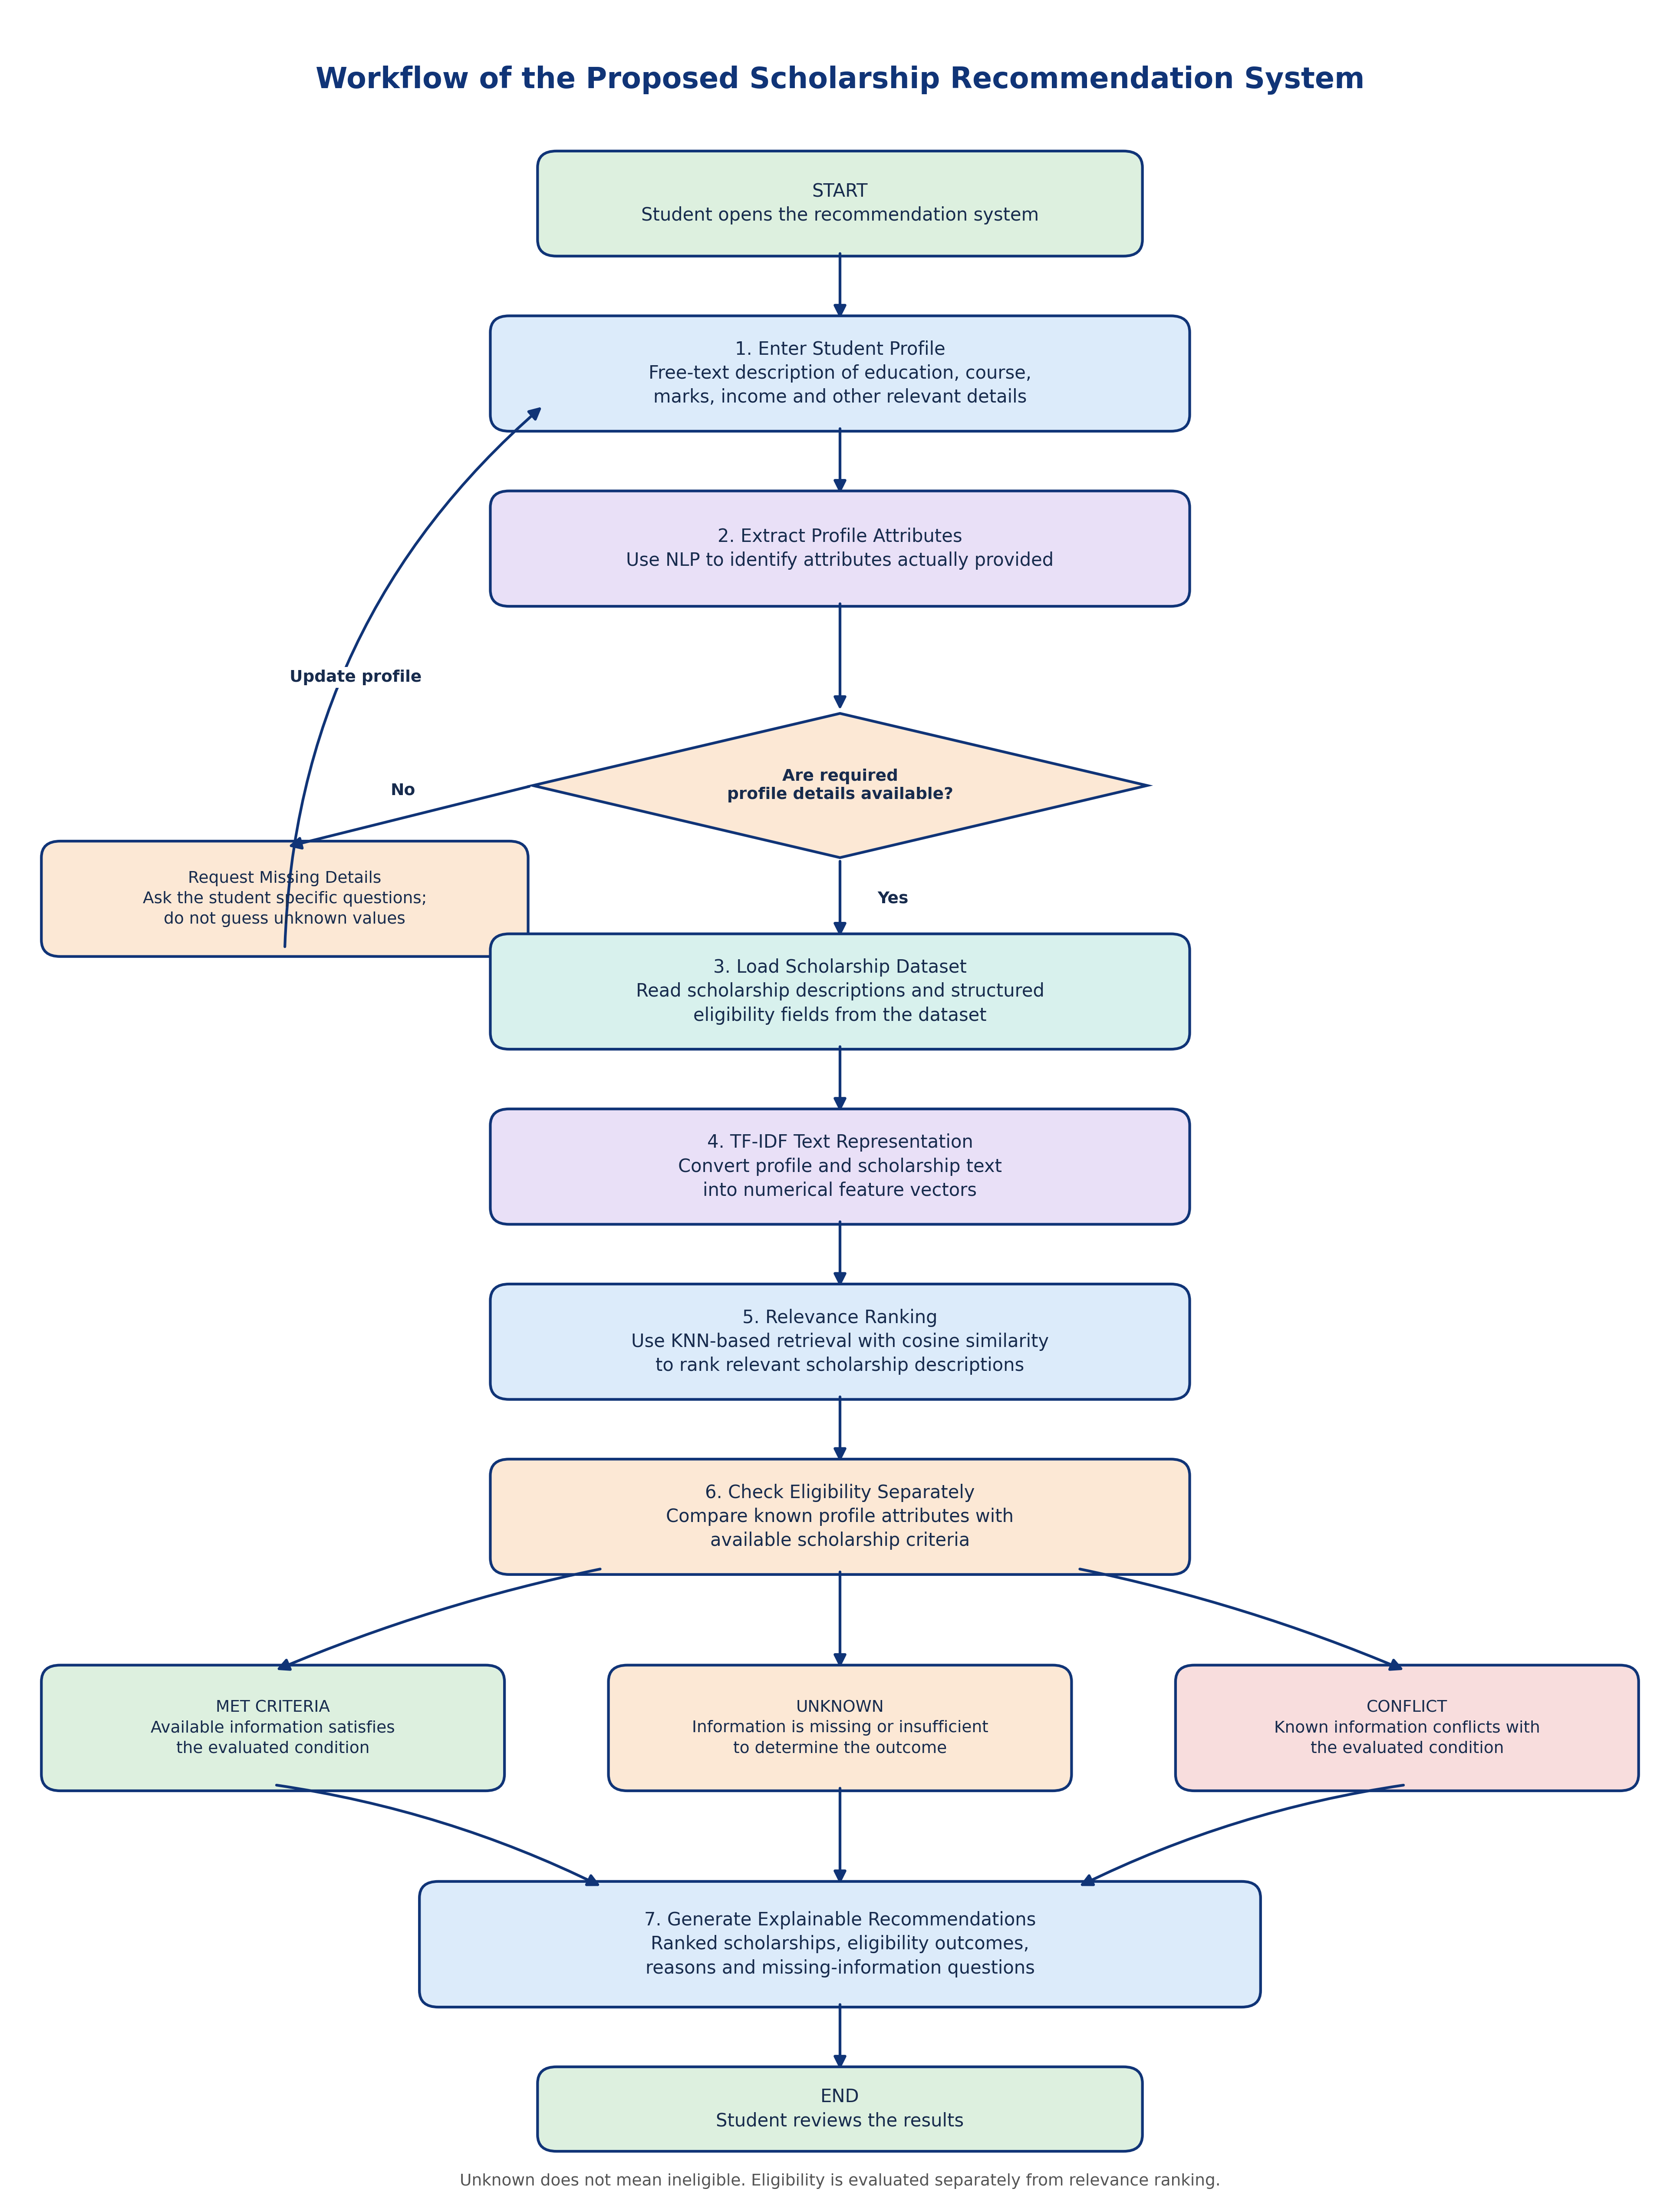
\includegraphics[width=0.94\textwidth]{system_architecture.png}
\caption{System architecture of the proposed scholarship recommendation and eligibility analysis system.}
\label{fig:architecture}
\end{figure*}

\subsection{Workflow}
Fig.~\ref{fig:workflow} shows the sequence from profile input to recommendation output. The system checks for missing details, represents scholarship descriptions, ranks relevant records, checks eligibility states, and explains the final results. Optional missing information should not block all recommendations; it should remain marked as unknown.
\begin{figure*}[!t]
\centering
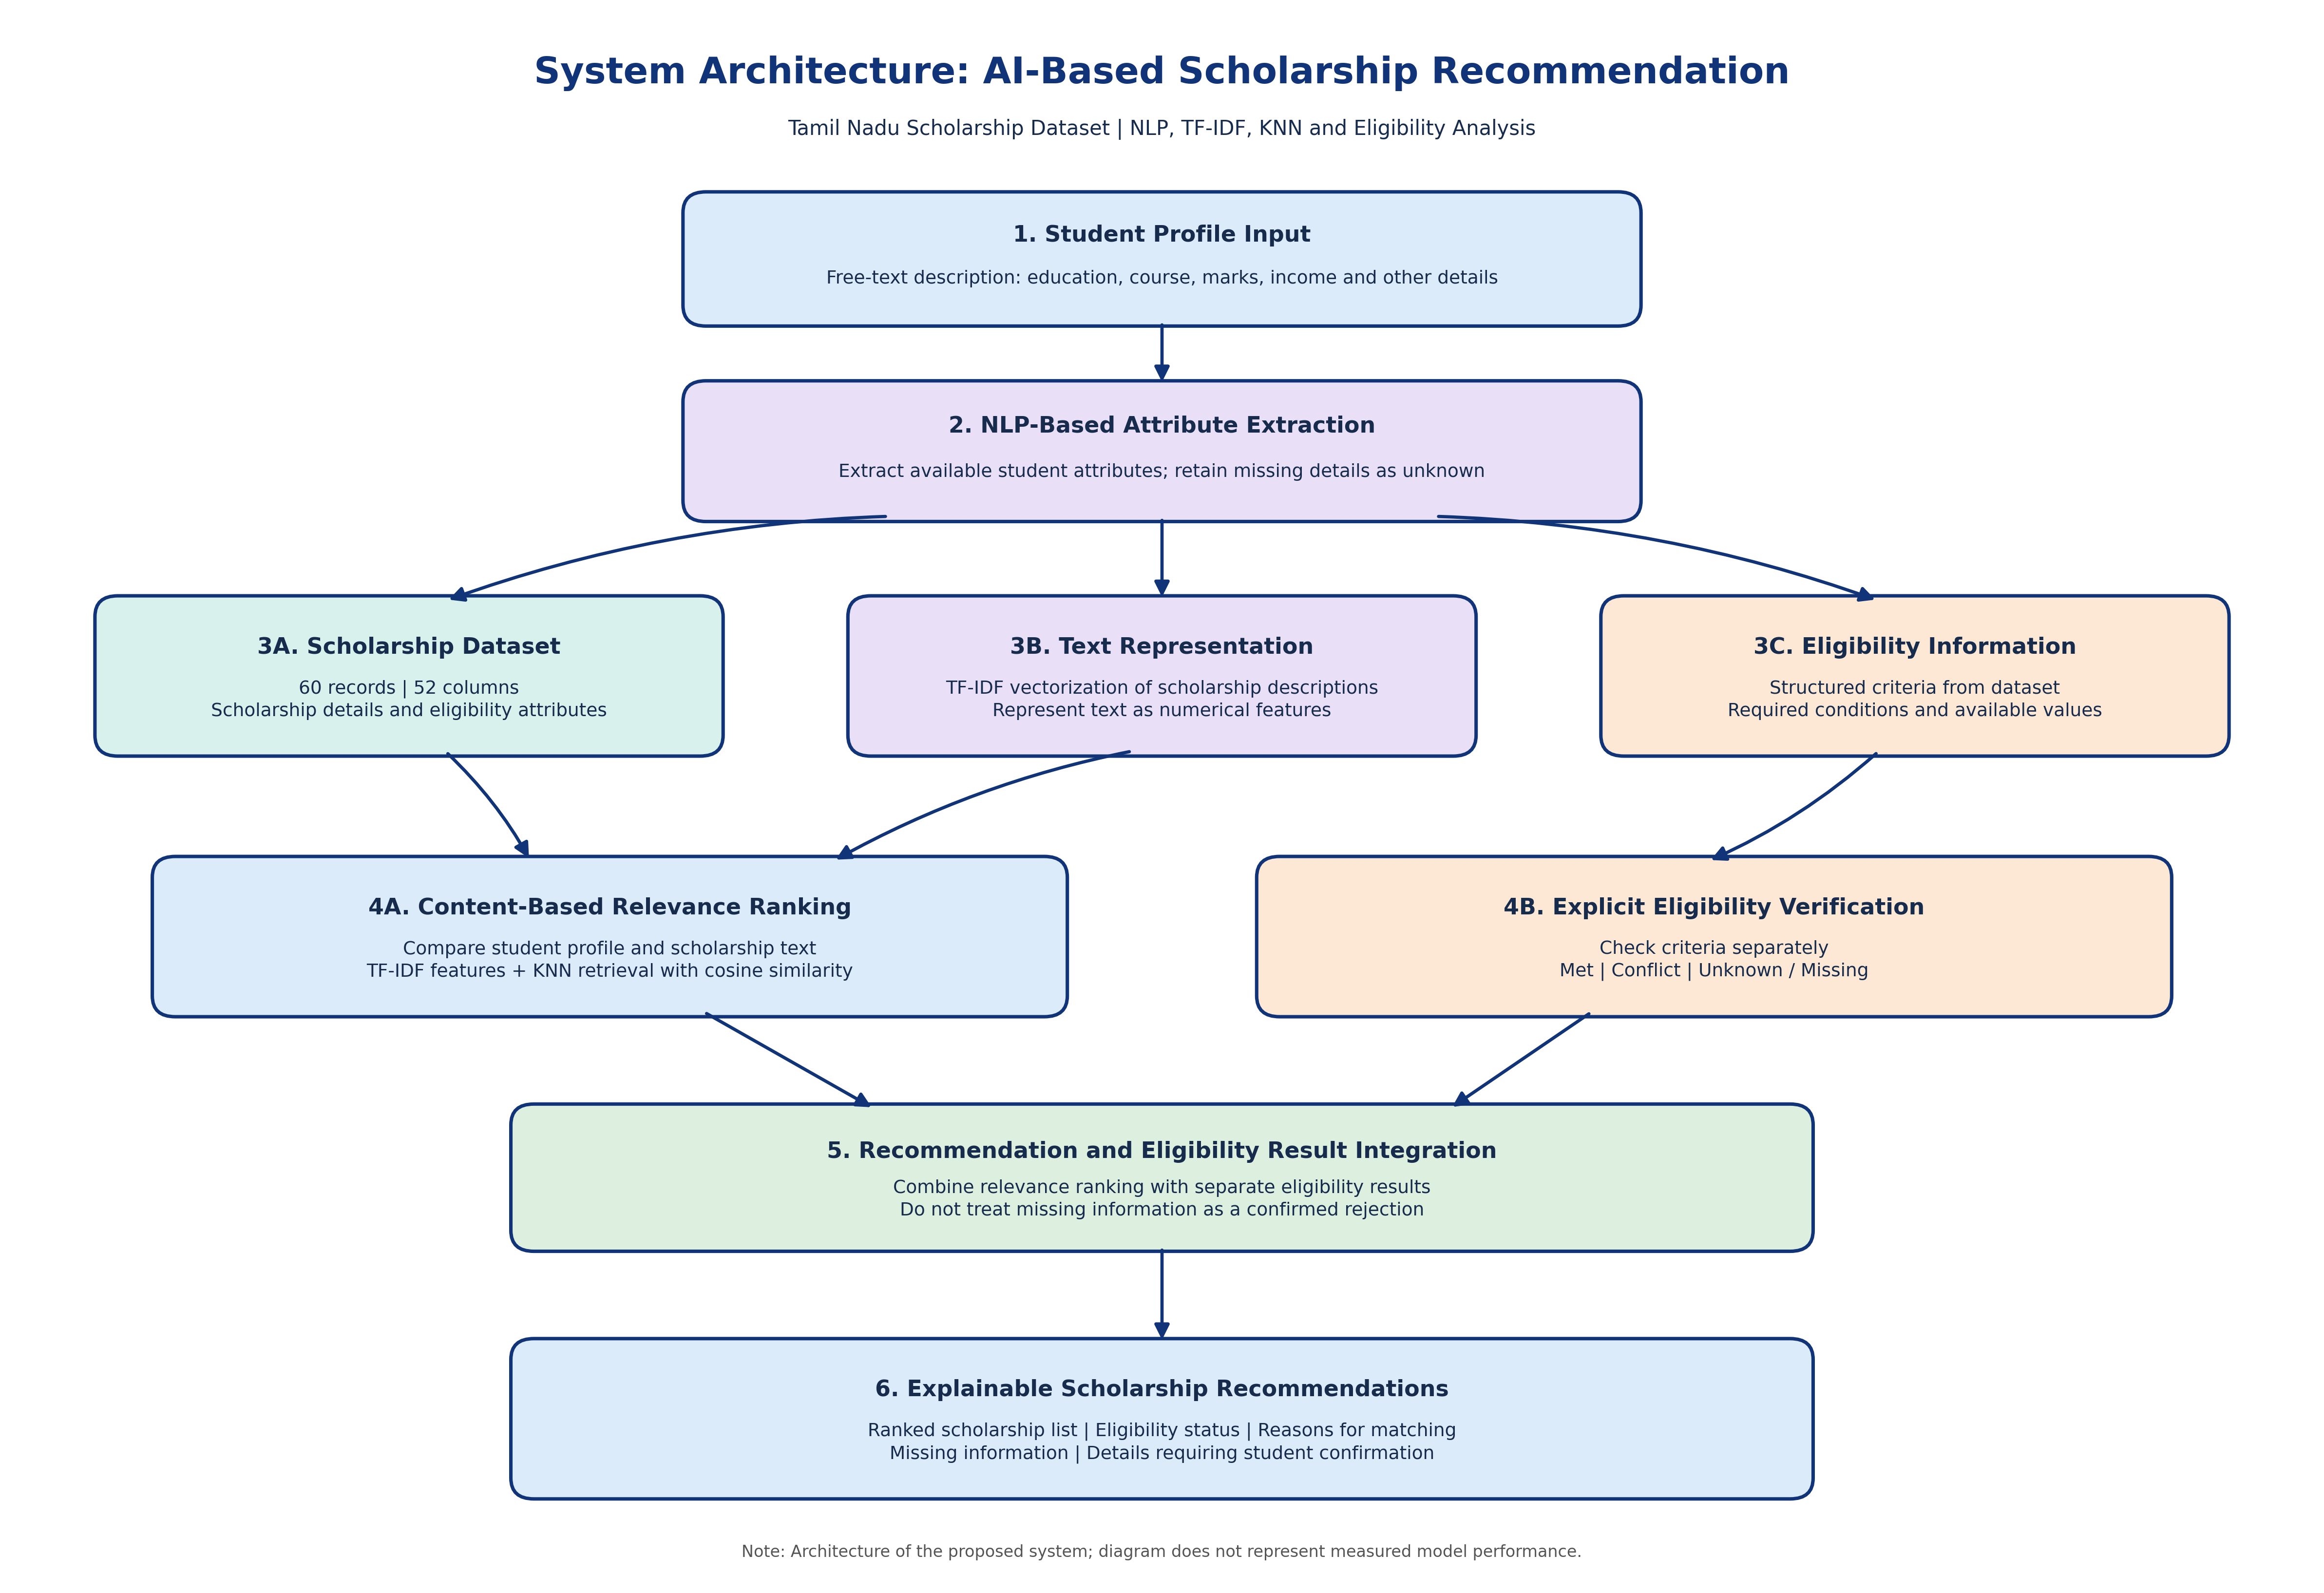
\includegraphics[width=0.96\textwidth]{workflow.png}
\caption{Workflow of the proposed scholarship recommendation and eligibility analysis process.}
\label{fig:workflow}
\end{figure*}

\section{Dataset Analysis and Figures}
Fig.~\ref{fig:types} shows the scholarship-type distribution derived from the current workbook. The chart retains the recorded category labels; categories are not silently merged. The diversity of labels indicates that the dataset contains different kinds of educational assistance and scholarship support.
\begin{figure}[!t]
\centering
\includegraphics[width=\columnwidth]{scholarship_type_distribution.png}
\caption{Distribution of recorded scholarship types in the Tamil Nadu scholarship dataset.}
\label{fig:types}
\end{figure}

Fig.~\ref{fig:eligibility} shows the number of records containing specific values in selected eligibility-related fields. The figure's ``specific value'' counts exclude blank entries and selected placeholder values according to the chart-generation procedure. They describe the presence of values, not official verification or confirmed student eligibility.
\begin{figure*}[!t]
\centering
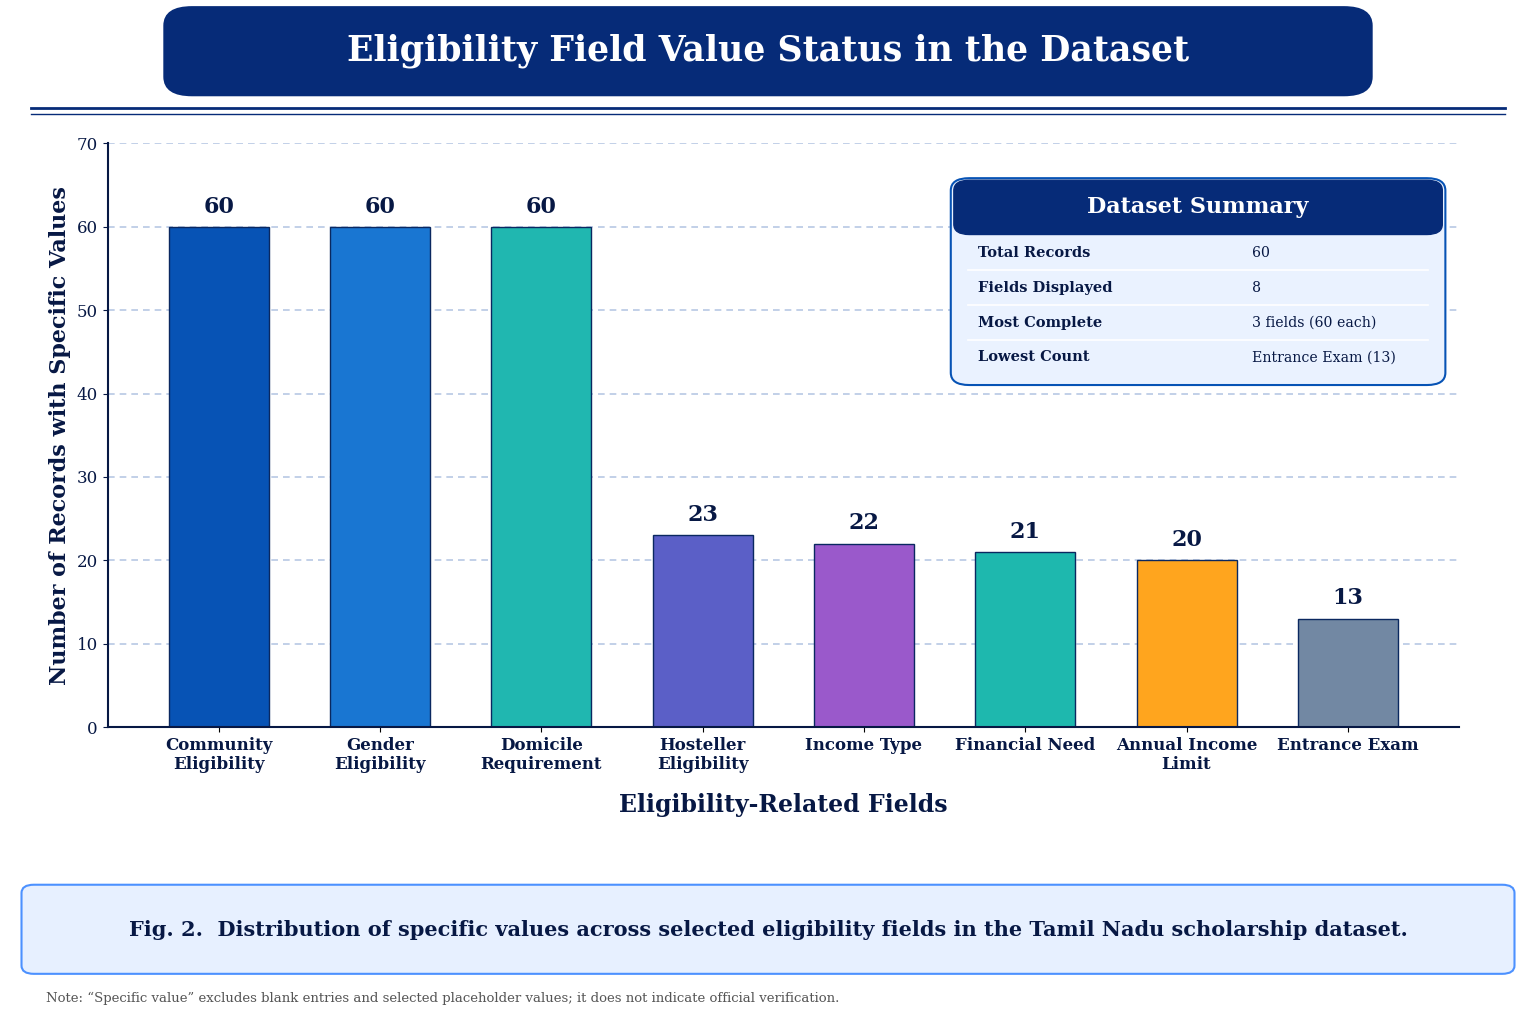
\includegraphics[width=0.94\textwidth]{eligibility_field_status.png}
\caption{Distribution of specific values across selected eligibility fields in the Tamil Nadu scholarship dataset.}
\label{fig:eligibility}
\end{figure*}

\section{Prototype Behaviour and Evaluation Considerations}
The intended prototype processes a free-text student profile, retrieves relevant scholarship records using TF--IDF and KNN cosine similarity, and checks the known profile attributes against each record's eligibility conditions. It then displays a ranked list with explicit explanations. This design is intended to reduce manual search effort and make uncertainty visible.

The currently available scholarship workbook does not contain labelled student--scholarship outcome pairs. Therefore, it does not by itself support a defensible claim of classification accuracy, precision, recall, F1-score, or award probability. Similarity values and hybrid ranking scores should be reported only as ranking indicators. A valid quantitative evaluation would require a separate set of student profiles and expert-verified relevance and eligibility labels. Suitable future retrieval measures could include Precision@K, Recall@K, Mean Reciprocal Rank, and Normalized Discounted Cumulative Gain, provided the corresponding relevance judgements are collected.

\subsection{Case-Study Evaluation Figure}
The supplied case-study evaluation image compares semantic-relevance ranking with a multi-state eligibility audit for five candidate opportunities. Its numerical values must be retained as experimental results only if they were generated by the actual implementation from a documented student profile and the current dataset. If the values are illustrative or manually created, this figure must be replaced with a verified output before submission.
\begin{figure*}[!t]
\centering
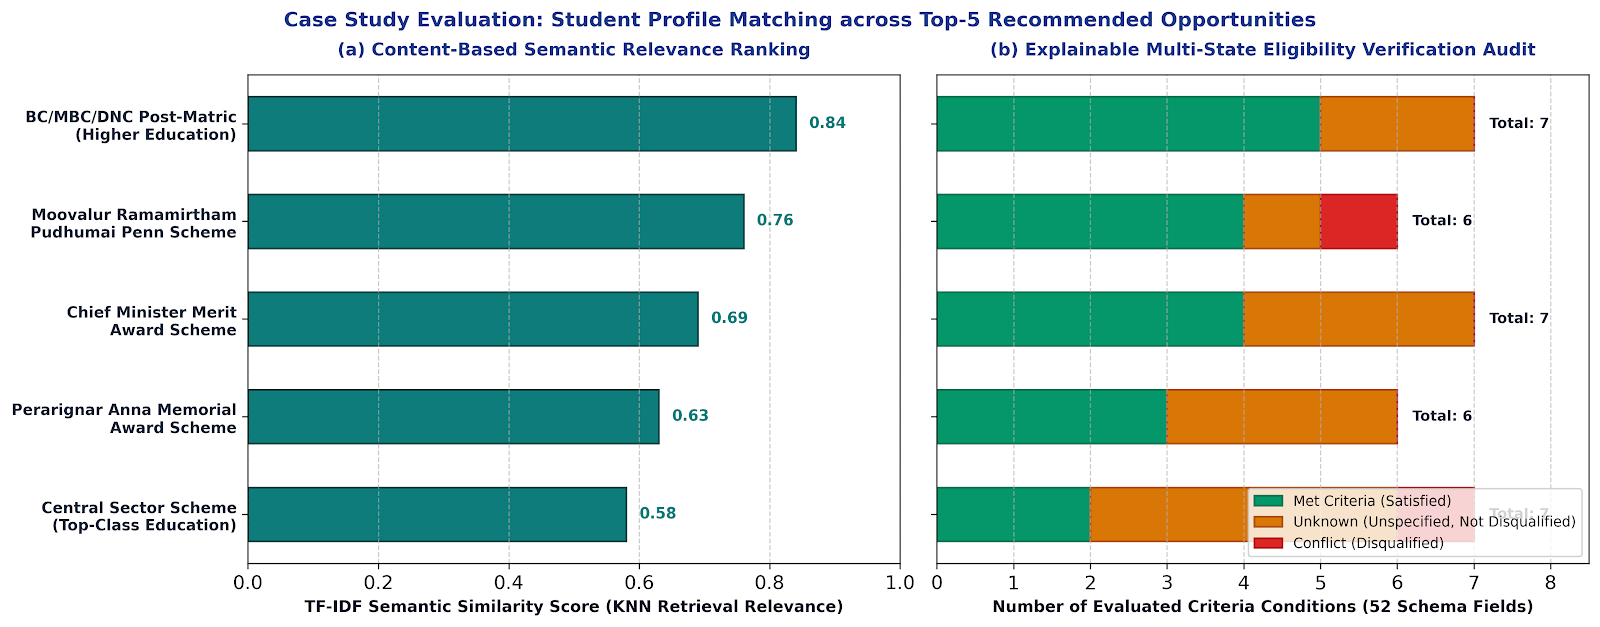
\includegraphics[width=0.96\textwidth]{case_study_evaluation.png}
\caption{Case-study visualisation of content-based relevance ranking and multi-state eligibility auditing. The displayed numerical values require confirmation against a reproducible prototype run before being treated as empirical results.}
\label{fig:caseeval}
\end{figure*}

\section{Results and Discussion}
The descriptive analysis establishes that the workbook contains 60 scholarship records with 52 columns and includes fields for scholarship identity, provider, education level, course category, benefits, eligibility descriptions, application information, source URLs, and academic year. The dataset includes multiple literal scholarship-type and education-level categories. Academic-year completeness is lower than that of several descriptive fields, and some eligibility values use free-text descriptions or placeholders.

These observations motivate a system that uses more than a single keyword and keeps eligibility checks explicit. TF--IDF and cosine similarity provide a transparent baseline for text retrieval, while the separate eligibility layer prevents text similarity from being mistaken for proof of eligibility. The prototype should be considered a retrieval and decision-support system rather than a supervised award-prediction model. No claim of improved accuracy or successful real-world award prediction is made from the descriptive dataset alone.

\section{Limitations and Future Work}
The current dataset contains 60 records and does not represent the complete scholarship ecosystem. Scholarship details, eligibility rules, and deadlines may change, so periodic checking against official sources is required. Some criteria are expressed as natural-language fields and may need improved rule parsing. Semantic similarity can identify relevant descriptions without guaranteeing that a student satisfies every administrative requirement.

Future work should expand the scholarship database, standardise the data schema, validate time-sensitive information, and develop a set of student profiles with expert-verified scholarship relevance and eligibility labels. The system could then be assessed using retrieval metrics and, where appropriate, classification metrics. Further improvements may include better multilingual profile processing, course-equivalence mapping, source-verification workflows, and clearer links to official application portals.

\section{Conclusion}
This paper presents a data-driven framework for scholarship recommendation and preliminary eligibility analysis focused initially on Tamil Nadu. The proposed method combines natural-language profile attribute extraction, TF--IDF text representation, KNN retrieval using cosine similarity, and explicit eligibility-condition matching. It distinguishes met, conflict, and unknown states so that missing information is not treated as a negative answer. The initial dataset contains 60 records and 52 columns and provides a starting point for scholarship discovery. Since labelled student--scholarship outcomes are not available in the dataset, ranking values must not be interpreted as model accuracy or award probabilities. The framework provides a basis for a more comprehensive and explainable recommendation tool after further data validation and evaluation.

\section*{Acknowledgment}
The authors may acknowledge the institution, project guide, and other contributors here, where applicable.

\begin{thebibliography}{00}
\bibitem{salton} G. Salton and C. Buckley, ``Term-weighting approaches in automatic text retrieval,'' \emph{Information Processing \& Management}, vol. 24, no. 5, pp. 513--523, 1988.
\bibitem{cover} T. M. Cover and P. E. Hart, ``Nearest neighbor pattern classification,'' \emph{IEEE Transactions on Information Theory}, vol. 13, no. 1, pp. 21--27, 1967.
\bibitem{manning} C. D. Manning, P. Raghavan, and H. Sch\"utze, \emph{Introduction to Information Retrieval}. Cambridge, U.K.: Cambridge University Press, 2008.
\bibitem{pedregosa} F. Pedregosa \emph{et al.}, ``Scikit-learn: Machine learning in Python,'' \emph{Journal of Machine Learning Research}, vol. 12, pp. 2825--2830, 2011.
\bibitem{tn_dce} Directorate of Collegiate Education, Government of Tamil Nadu, ``Scholarship.'' [Online]. Available: \url{https://tndce.tn.gov.in/Home/scholarship}
\bibitem{tn_bc} Government of Tamil Nadu, Backward Classes, Most Backward Classes and Denotified Communities Welfare Department, ``Welfare Schemes.'' [Online]. Available: \url{https://www.bcmbcmw.tn.gov.in/welfschemes.htm}
\bibitem{tn_dap} Government of Tamil Nadu, Department for the Welfare of Differently Abled Persons, ``Special Education and Financial Assistance.'' [Online]. Available: \url{https://www.scd.tn.gov.in/specialedu.php}
\end{thebibliography}

\balance
\end{document}
